%%%%%%%%%%%%%%%%%%%%%%%%%%%%%%%%%%%%%%%%%
% University Assignment Title Page 
% LaTeX Template
% Version 1.0 (27/12/12)
%
% This template has been downloaded from:
% http://www.LaTeXTemplates.com
%
% Original author:
% WikiBooks (http://en.wikibooks.org/wiki/LaTeX/Title_Creation)
%
% License:
% CC BY-NC-SA 3.0 (http://creativecommons.org/licenses/by-nc-sa/3.0/)
% 
% Instructions for using this template:
% This title page is capable of being compiled as is. This is not useful for 
% including it in another document. To do this, you have two options: 
%
% 1) Copy/paste everything between \begin{document} and \end{document} 
% starting at \begin{titlepage} and paste this into another LaTeX file where you 
% want your title page.
% OR
% 2) Remove everything outside the \begin{titlepage} and \end{titlepage} and 
% move this file to the same directory as the LaTeX file you wish to add it to. 
% Then add \input{./title_page_1.tex} to your LaTeX file where you want your
% title page.
%
%%%%%%%%%%%%%%%%%%%%%%%%%%%%%%%%%%%%%%%%%
%\title{Title page with logo}
%----------------------------------------------------------------------------------------
%	PACKAGES AND OTHER DOCUMENT CONFIGURATIONS
%----------------------------------------------------------------------------------------
\documentclass[UTF-8,12pt]{article}
\usepackage[UTF8]{ctex}
\usepackage[english]{babel}
\usepackage[utf8x]{inputenc}
\usepackage{amsmath}
\usepackage{graphicx}
\usepackage{hyperref}
\usepackage[colorinlistoftodos]{todonotes}

\begin{document}

\begin{titlepage}

\newcommand{\HRule}{\rule{\linewidth}{0.5mm}} % Defines a new command for the horizontal lines, change thickness here

\center % Center everything on the page
 
%----------------------------------------------------------------------------------------
%	HEADING SECTIONS
%----------------------------------------------------------------------------------------

\textsc{\LARGE \bfseries 中山大学 }\\[0.3cm] % Name of your university/college
\textsc{\Large 数据科学与计算机学院}\\[0.5cm] % Major heading such as course name
\textsc{\Large 软件工程}\\[0.3cm] % Major heading such as course name
\textsc{\Large 人工智能}\\[0.5cm]
 % Minor heading such as course title

%----------------------------------------------------------------------------------------
%	TITLE SECTION
%----------------------------------------------------------------------------------------

\HRule \\[0.4cm]
{ \huge \bfseries BP 神经网络算法实验报告}\\[0.03cm] % Title of your document
\HRule \\[1.5cm]

 
%----------------------------------------------------------------------------------------
%	AUTHOR SECTION
%----------------------------------------------------------------------------------------

\begin{minipage}{0.4\textwidth}
\begin{flushleft} \large
\emph{Submitted By:}\\
熊永琦 16340258\\
徐伟元 16340261\\
李天译 16340122
\end{flushleft}
\end{minipage}
~
\begin{minipage}{0.5\textwidth}
\begin{flushright} \large
\emph{Submitted To:} \\
王甲海\\ 教授\\ 大数据与计算智能研究所 % Supervisor's Name
\end{flushright}
\end{minipage}\\[1cm]

% If you don't want a supervisor, uncomment the two lines below and remove the section above
%\Large \emph{Author:}\\
%John \textsc{Smith}\\[3cm] % Your name

%----------------------------------------------------------------------------------------
%	DATE SECTION
%----------------------------------------------------------------------------------------

{\large 2019-1-10}\\[1cm] % Date, change the \today to a set date if you want to be precise

%----------------------------------------------------------------------------------------
%	LOGO SECTION
%----------------------------------------------------------------------------------------


\includegraphics[width=2in]{logo.png}\\[0.5cm] % Include a department/university logo - this will require the graphicx package
 
%----------------------------------------------------------------------------------------

\vfill % Fill the rest of the page with whitespace

\end{titlepage}


\begin{abstract}
    
本实验利用 BP 神经网络算法,完成了对于单个手写数字的识别,识别准确率达到了 95\% 以上。

\end{abstract}

\section{实验题目}

构造一个三层的BP神经网络,完成手写0-9数字的识别:

\begin{enumerate}
    \item 设计网络的结构,比如层数,每层的神经元数,单个神经元的输入输出函数
    \item 根据数字识别的任务,设计网络的输入和输出
    \item 实现BP网络的错误反传算法,完成神经网络的训练和测试,最终识别率达到70\%以上
    \item 数字识别训练集可以自己手工制作,也可以网上下载
\end{enumerate}

\section{BP 神经网络原理}

BP(Back Propagation)神经网络的学习过程由信号的正向传播与误差的反向传播两个过程组成。正向传播时,输入样本从输入层传入,经隐层逐层处理后,传向输出层。若输出层的实际输出与期望输出不符,则转向误差的反向传播阶段。误差的反向传播是将输出误差以某种形式通过隐层向输入层逐层反传,并将误差分摊给各层的所有单元,从而获得各层单元的误差信号,此误差信号即作为修正各单元权值的依据。

\subsection{正向传播阶段}

具体到单个神经元(隐含层和输出层)来讲,其计算过程如 Figure 1 所示。

\begin{figure}
    \centering
    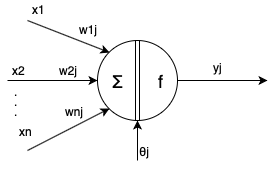
\includegraphics{single.png}
    \caption{单个神经元的运算流程}
    \label{fig:single}
\end{figure}

对于每个输入的值,我们乘上一个加权比重 $w_{ij}$,然后将其求和,再加上一个偏移量($\theta_j$),就得到了该神经元的值。为什么我们这里需要一个偏移呢?考虑一个我们都知道的式子:

$$y = kx + b$$

在神经网络算法中,权重 $w$ 扮演的实际上就是 k 的角色,它决定了整个超平面在解空间中的方向,而偏移量(bias)就是决定了超平面和坐标轴的交点位置,否则我们的超平面将永远从原点出发。

总而言之,我们需要首先求得神经元上的值。考虑一个三层神经网络(一层输入层,一层隐含层,一层输出层),输入层的输出即是输入的值,记作 $x_i$。隐含层输出记为 $H_j$,输出层输出记为 $O_k$。我们假设输入层的神经元数为 n,隐含层的神经元数为 l,有如下式子:

$$H_j=f(\sum_{i=1}^nw_{ij}x_i+a_j)$$
$$O_k=f(\sum_{i=1}^lw_{jk}H_j+b_k)$$

其中 $a$ 和 $b$ 分别是隐含层和输出层的偏移量,$f$ 为激活函数,此处我们选用的是 Logistics 函数。特别的,在处理输出层神经元的时候,我们不会对其进行激活函数处理。

\subsection{反向传播阶段}

在训练阶段,每次完成了正向传播后,我们需要将得到的估计值与实际情况的真实值进行比对,并且通过反向传播这个误差来达到修正整个神经网络的效果。

\subsubsection{激活函数 Logistics}

在前面,我们提到了 Logistics 函数,其是一个值域为 (0,1) 的函数。这使得它非常适合作为激活函数使用,它将所有输入数据都归一化了。Logistics 函数另一个优良的性质来源于它的表达式,其表达式和导数如下:

$$f(x)=\frac{1}{1+e^{-x}}$$
$$f^{'}(x)=\frac{1-e^{-x}}{1+e^{-x}}$$

这个漂亮的导数式将给我们的后续计算带来很多便利。

\subsubsection{计算误差}

设实际值的向量为 $Y$,则结合前文得到的输出层输出向量 $O$ 的表达式,假设输出层神经元数量为 $m$ 我们可以定义误差公式如下:

$$e_k=Y_k-O_k$$
$$E=\frac12\sum^m_{k=1}e_k^2$$

之所以使用平方和,是因为作为整体存在时,单个 e 的方向是不重要的,我们需要的是偏离的程度的和来评判当前神经网络的准确程度。在后面对其求偏导的时候,我们自然可以通过 e 得到误差的方向信息。

\subsubsection{更新权值和偏置}

在 BP 神经网络中,我们使用的是梯度下降法来选择一个更优的权值和偏置。顾名思义,我们考虑 E 对于权值或者偏置的偏导,这样就获得了误差 E 在某个权或偏置的维度上的最快下降方向,将这个值和我们设置的学习步长 $\eta$ 相乘,即可获得我们需要的权值的变化量。

更具体的来讲,以权值为例,我们首先计算误差对于隐含层到输出层的权重的偏导:

$$\frac{\partial E}{\partial w_{jk}}=\sum_{k=1}^m(Y_k - O_k)(-\frac{\partial O_k}{\partial w_{jk}})=(Y_k-O_k)(-H_j)=-e_kH_j$$

因为我们希望尽可能减少误差 E,所以我们采用逆梯度方向进行梯度下降,即:

$$
\begin{aligned}
    w_{jk}&=w_{jk}-\frac{\partial E}{\partial w_{jk}}\\
    &=w_{jk}+\eta e_kH_j
\end{aligned}
$$

同理,我们下面计算输入层到隐含层的权值更新。首先求得计算误差对于输入层到隐含层的权重的偏导,根据链式法则,我们有:

$$\frac{\partial E}{\partial w_{ij}}=\frac{\partial E}{\partial H_j}\cdot\frac{\partial H_j}{\partial w_{ij}}$$

故我们首先分别求 $\frac{\partial E}{\partial H_j}$ 和 $\frac{\partial H_j}{\partial w_{ij}}$ 的表达式:

$$
\begin{aligned}
    \frac{\partial E}{\partial{H_j}} &= \sum_{k=1}^m(Y_k - O_k)(-\frac{\partial O_k}{\partial H_j})\\
    &=-\sum_{k=1}^m(Y_k - O_k)w_{jk}\\
    &=-\sum_{k=1}^me_kw_{jk}
\end{aligned}
$$

$$
\begin{aligned}
    \frac{\partial H_j}{\partial w_{ij}}&=\frac{\partial f(\sum_{i=1}^nw_{ij}x_i+a_j)}{\partial w_{ij}}\\
    &=f(\sum_{i=1}^nw_{ij}x_i+a_j)\cdot[1-f(\sum_{i=1}^nw_{ij}x_i+a_j)]\cdot\frac{\partial(\sum_{i=1}^nw_{ij}x_i+a_j)}{\partial w_{ij}}\\
    &=H_j(1-H_j)x_i
\end{aligned}
$$

最后,我们得到输入层到隐含层的权值的更新公式:

$$
\begin{aligned}
    w_{ij}&=w_{ij}+\eta\cdot\frac{\partial E}{\partial{H_j}}\cdot\frac{\partial H_j}{\partial w_{ij}}\\
    &=w_{ij}+\eta H_j(1-H_j)x_i\sum_{k=1}^mw_{jk}e_k
\end{aligned}
$$

所以,我们最后得到权值的更新公式为:

$$
\left\{
\begin{aligned}
    w_{ij}&=&w_{ij}+\eta H_j(1-H_j)x_i\sum_{k=1}^mw_{jk}e_k\\
    w_{jk}&=&w_{jk}+\eta e_kH_j
\end{aligned}
\right.
$$

上式的计算次序不可改变,因为输入层到隐含层的权值依赖于隐含层到输出层的权值的初始值。

对于偏置(即偏移量)的讨论是类似的,因为我们可以在正向传播的过程中看到,偏置参与计算的过程实际上和权值类似,只是没有和输入值相乘而已。反映到最后的结果上也是如此,这里不做多余的推导(这和权值类似),直接给出最后的更新式:

$$
\left\{
\begin{aligned}
    a_j&=&a_j+\eta H_j(1-H_j)\sum_{k=1}^mw_{jk}e_k\\
    b_k&=&b_k+\eta e_k
\end{aligned}
\right.
$$

值得注意的是,和前面的权值更新相同,两个式子的计算次序不可颠倒,其理由也是类似的。

\subsubsection{算法优化}

如果单纯利用上面的公式进行网络参数更新,我们的确可以写出一个可正确运行的 BP 神经网络,但是这显然不会是一个好用的软件。因为上面的所有公式均是串行的,计算代价非常高,并且由于我们使用 Python 来进行计算,这种低效率的算法会严重影响程序使用体验。

基于上述原因,我们使用矩阵运算等价改写了上述的式子,利用 Numpy 来实现矩阵运算的并行化加速,并最终实现了约 100 倍的运行时间优化,这使得我们拥有更宽泛的参数选择空间,从而在相同时间内达到更好的算法效果。这部分的具体实现请参见我们仓库内的 \underline{\href{https://github.com/xwy27/ArtificialIntelligenceProjects/blob/master/AI_Web/NumRecognition/model/neuralNetwork.py}{neuralNetwork.py}} 文件。

\newpage
\section{神经网络结构设计}

一个典型的三层 BP 神经网络结构如 Figure 2 所示,由一个含若干神经元的输入层,一个含若干神经元的隐含层和一个含若干神经元的输出层构成。

\begin{figure}
    \centering
    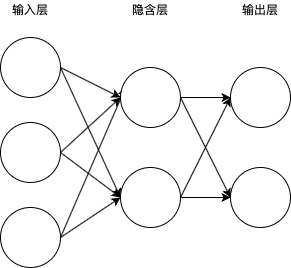
\includegraphics{BP.png}
    \caption{神经网络结构}
    \label{fig:BP}
\end{figure}

在最初的设计中,我们为输入层引入了与待识别图片像素个数相同的节点,并求第一层节点数的平方根作为隐含层的节点数,最后只留一个输出层节点,直接输出识别出的数字本身。

但是这种设计存在显著的问题:对于一个给定的正确答案,不同的错误答案造成的误差不相等。或者更具体一点,不同的错误答案对于修正的力度的影响不一。

这个问题听上去有点难以理解,让我们举个例子:假设我们的正确答案为 3,而一个错误答案为 1,另一个错误答案为 9。那么第一个错误答案的 E 为 2,第二个错误答案的 E 为 18。这乍一看上去是没有问题的,因为 9 的确会比 1 和 3 「相差得更多一些」。但让我们好好研读一下实验的目的:输出手写数字对应的数字。我们输出的数字和正确数字的差值不是我们关心的内容,正确与否才是我们唯一关心的事情。换句话说,无论错误答案是 1 还是 9,他们提供的误差都应该是相同的,在这个问题里面没有错误程度可言。

事实上也是如此,这种不合理的结构的神经网络最后给出的结果是难以接受的,在我们反复尝试后,它的正确率也没能超过 50\%。

为此,我们更改了我们的设计——将输出层调整为 10 个神经元\cite{op},第 k 个神经元输出的含义为 “当前数字为 k 的可能性有多大”。因此整个神经网络最后判定的结果是 “可能性最大的节点是哪一个”,那么神经网络就认为当前输入的数字是可能性最大的节点的编号。

在这种情况下,我们的标准输出是一个向量,其中正确数字作为序号所指向的元素的值为 1,其余元素为 0。

这种结构收获了非常好的结果,我们将在测试与结论一节里详细阐述。

\section{测试及结论}

\subsection{数据选择}

一个完整的手写数字识别程序需要做的事情非常多,包括数字识别,对象居中,降噪处理等等。但是这写问题主要是数字图像领域的知识,偏离了人工智能项目的初衷。因而我们选择了 MNIST 数据集\cite{MNIST}作为我们的训练数据和测试数据。

MNIST 数据集是手写数字的数据库,其训练集内包含了 60000 个样例,测试集内包含了 10000 个样例,他们来自超过 250 位测试者的手写字体。这些数字图片的尺寸都被统一为 28 * 28。非常适合用于纯粹的 BP 神经网络算法测试

\subsection{运行结果}

\begin{figure}
    \centering
    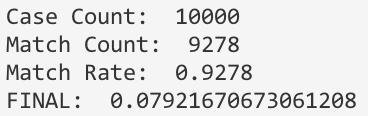
\includegraphics{BP-Test.png}
    \caption{测试结果}
    \label{fig:BP Test}
\end{figure}


我们使用 144 个隐含层,0.0003 的学习步长进行训练和测试,其最终测试集识别率能达到 92.78\%,远远超过了题目要求的 70\% 识别率。

另外,我们还训练了一个包含更多隐含层的配置文件,该文件也是通过训练集训练得到,直接使用此文件可以达到 95.97\% 的识别率,同样远超题目要求的 70\% 识别率。

\subsection{结论}

BP 神经网络算法能够很好地解决手写数字识别的问题。在 BP 神经网络中,网络结构和输出向量含义的设计至关重要,一个好的网络结构设计能够让准确率提升数个档次。另外,学习步长的选择也非常关键,在我们的测试过程中,我们还遇到过因为步长过长,导致神经网络算法无法正常收敛的情况。

因为我们通过将图片像素拉成向量进行输入的过程中损失了像素之间的位置关系信息,从拓展上来讲,我们还可以考虑在 BP 神经网络中结合卷积神经网络的思想(保留位置信息)来进一步提高准确率。

\begin{thebibliography}{}
\bibitem{op} https://medium.com/analytics-vidhya/neural-networks-for-digits-recognition-e11d9dff00d5
\bibitem{MNIST} http://yann.lecun.com/exdb/mnist/
\end{thebibliography}

\end{document}